

\section{Method}\label{sec:algorithm} 

\subsection{Data Processing and Undersampling Simulation}
To train our reconstruction networks, we first need to simulate the k-space undersampling process that occurs in accelerated clinical MRI scans. As illustrated in Figure \ref{fig:undersampling}, we start with fully sampled 2D image slices. We apply a 2D Fast Fourier Transform (FFT) to convert these images into the frequency domain (k-space). Subsequently, we generate a 2D random variable-density undersampling mask with a specific acceleration factor (e.g., $5\times$). This mask is applied to the fully sampled k-space data to simulate the acquisition process. Finally, an Inverse Fast Fourier Transform (IFFT) is applied to the undersampled k-space data to obtain the zero-filled, aliased images, which serve as the inputs to our deep learning models.

\begin{figure}[h]
    \centering
    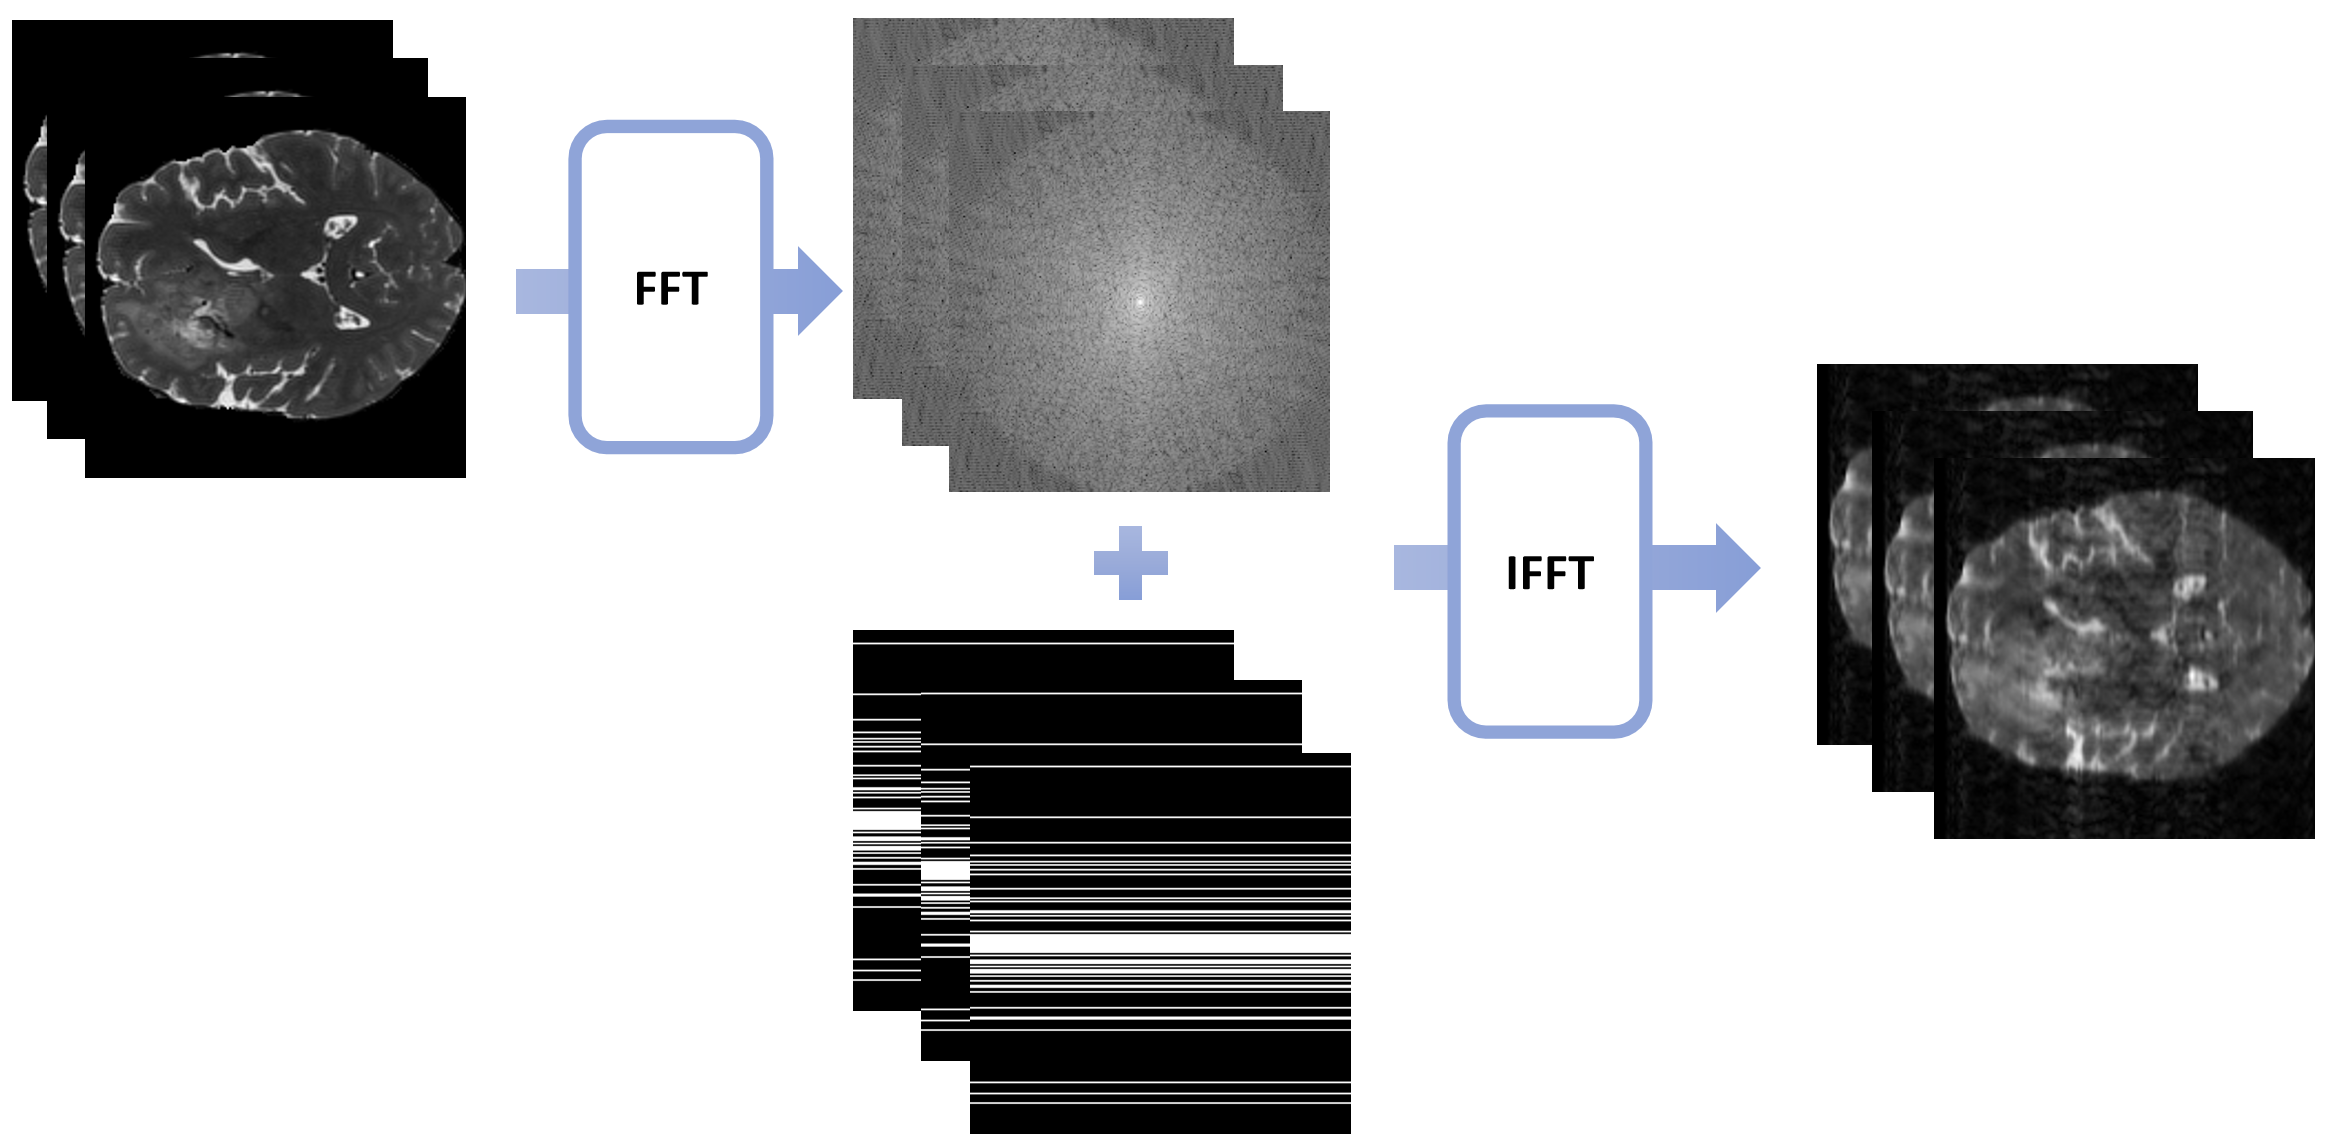
\includegraphics[width=\linewidth]{figures/data.png}
    \caption{Pipeline of the data preprocessing and undersampling simulation}
    \label{fig:undersampling}
\end{figure}

\subsection{Baseline Reconstruction Network (Task 2)}
In the initial phase of our project, we formulated the MRI reconstruction as an image-to-image translation problem and developed a baseline model based on the U-Net architecture, as shown in Figure \ref{fig:task2_unet}. The network takes the blurred, undersampled MRI image as input and processes it through a symmetric encoder-decoder structure. 

The encoder progressively downsamples the spatial resolution while increasing the channel depth using DoubleConv blocks (a sequence of $3\times3$ Convolution, Batch Normalization, and ReLU activation) followed by Max Pooling layers. A bottleneck layer captures the deepest latent representations. The decoder then progressively upsamples the feature maps using Transposed Convolutions and fuses them with high-resolution features from the encoder via skip connections. A final $1\times1$ convolution maps the deep features back to a single-channel reconstructed MRI image.
\begin{figure*}[t] 
	\begin{center} 
		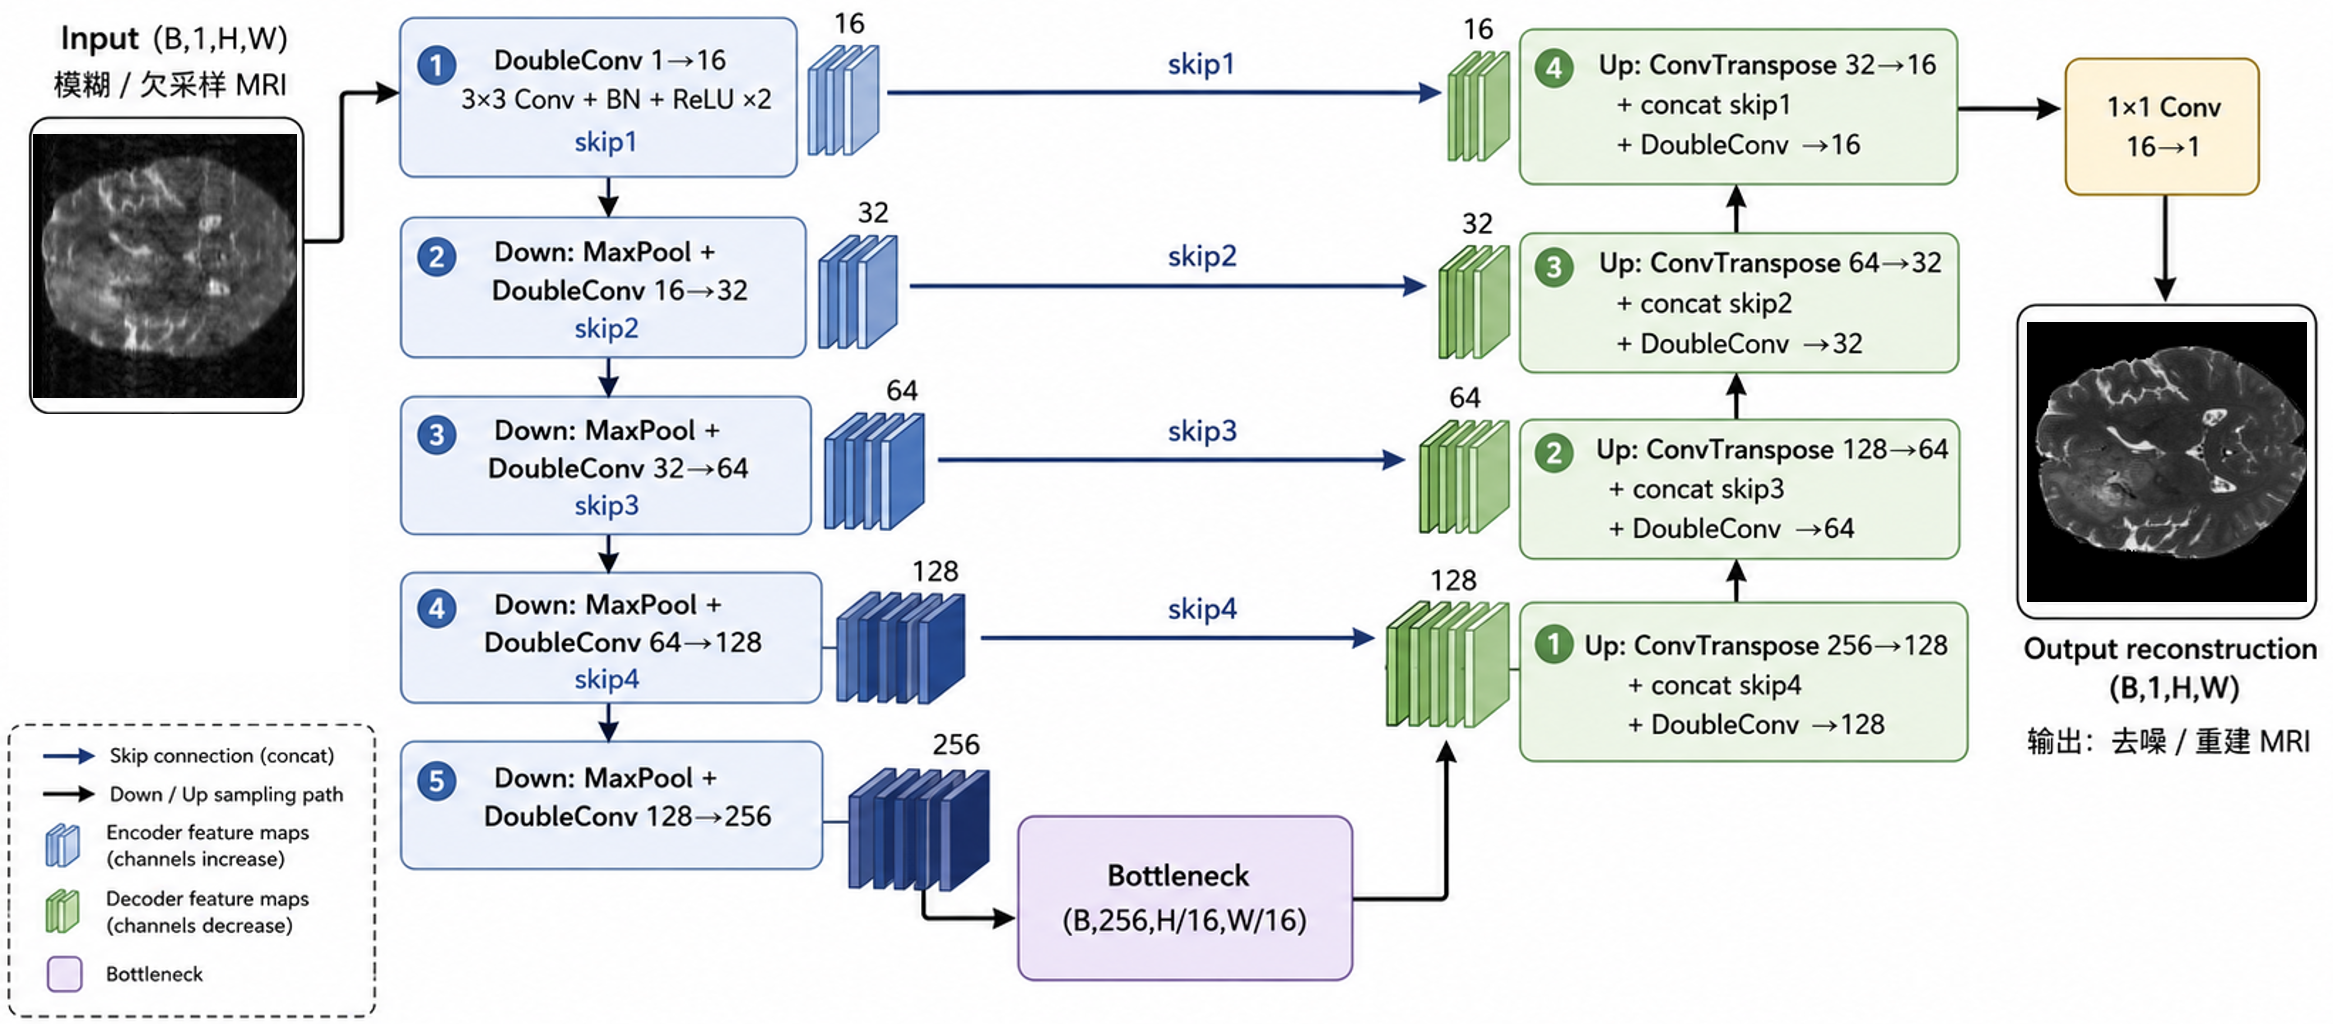
\includegraphics[width=\linewidth]{figures/pipeline_1.png} 
	\end{center} 
    \vspace{-20pt}  
	\caption{Overall pipeline of the baseline U-Net architecture (Task 2), which employs a symmetric encoder-decoder structure with skip connections to reconstruct high-quality, aliasing-free MRI images from undersampled T2 inputs.}
	\label{fig:task2_unet} 
	\vspace{-15pt}
\end{figure*} 


\subsection{Multi-modal Fusion and Unrolled Reconstruction (Task 3)}
To further elevate the reconstruction quality to a clinical grade, we advanced our architecture to a Multi-modal Unrolled Reconstruction Network (Figure \ref{fig:task3_pipeline}). This advanced pipeline leverages the fully sampled T1 modality to guide the reconstruction of the highly undersampled T2 modality.

The architecture consists of three core components:
\begin{enumerate}
    \item \textbf{Feature Fusion Module:} We utilize shallow CNN encoders to extract features from both the aliased T2 image and the fully sampled T1 image. A Cross-Attention mechanism is introduced where the T2 features act as the \textit{Query}, and the T1 features act as the \textit{Key} and \textit{Value}. This allows the network to borrow structural priors from the T1 image to complement the missing information in T2.
    \item \textbf{Unrolled Block:} The fused features are fed into a cascade of iterative unrolled blocks. Each block mimics an iteration of traditional optimization algorithms, containing a CNN Denoiser/Regularizer to refine the image features recursively.
    \item \textbf{Data Consistency (DC) Layer:} To ensure fidelity to the originally acquired data, a DC layer is appended after each unrolled iteration. It transforms the intermediate prediction back to the k-space, replaces the predicted values at sampled positions with the actual measured k-space data, and transforms it back to the image domain.
\end{enumerate} 

\subsection{Loss Function Design}
Traditionally, MRI reconstruction models are optimized using solely the Mean Squared Error (MSE) loss. However, relying purely on pixel-wise loss functions often leads to over-smoothed results. To mitigate this and enhance both the structural fidelity and visual quality, we formulated a comprehensive hybrid loss function combining MSE, Wavelet, and Perceptual losses:
\begin{equation}
\begin{split}
    \mathcal{L}_{total} &= \lambda_{mse}\mathcal{L}_{MSE}(x, \hat{x}) \\
    &\quad + \lambda_{wavelet}\mathcal{L}_{Wavelet}(x, \hat{x}) \\
    &\quad + \lambda_{perceptual}\mathcal{L}_{LPIPS}(x, \hat{x})
\end{split}
\end{equation}
where $x$ is the ground truth fully sampled image, $\hat{x}$ is the reconstructed image, and $\lambda$ represents the balancing weights for each respective component.

\textbf{Wavelet Loss ($\mathcal{L}_{Wavelet}$):} We introduced a wavelet-domain loss to explicitly penalize the loss of high-frequency details. By decomposing the images into four frequency bands using the Discrete Wavelet Transform, we calculate the $L_1$ distance for each band separately:
\begin{equation}
\begin{split}
    \mathcal{L}_{wavelet} &= w_{LL}\|LL_x - LL_{\hat{x}}\|_1 + w_{LH}\|LH_x - LH_{\hat{x}}\|_1 \\
    &\quad + w_{HL}\|HL_x - HL_{\hat{x}}\|_1 + w_{HH}\|HH_x - HH_{\hat{x}}\|_1
\end{split}
\end{equation}
Here, the $LL$ band preserves the global contrast and basic structure (low-frequency), while the $LH$, $HL$, and $HH$ bands extract high-frequency details along the horizontal, vertical, and diagonal directions, respectively. As illustrated in Figure \ref{fig:wavelet_vis}, analyzing the error maps of these decomposed bands allows the network to precisely target and recover fine structural edges that are often blurred by standard MSE loss.

\begin{figure}[h]
    \centering
    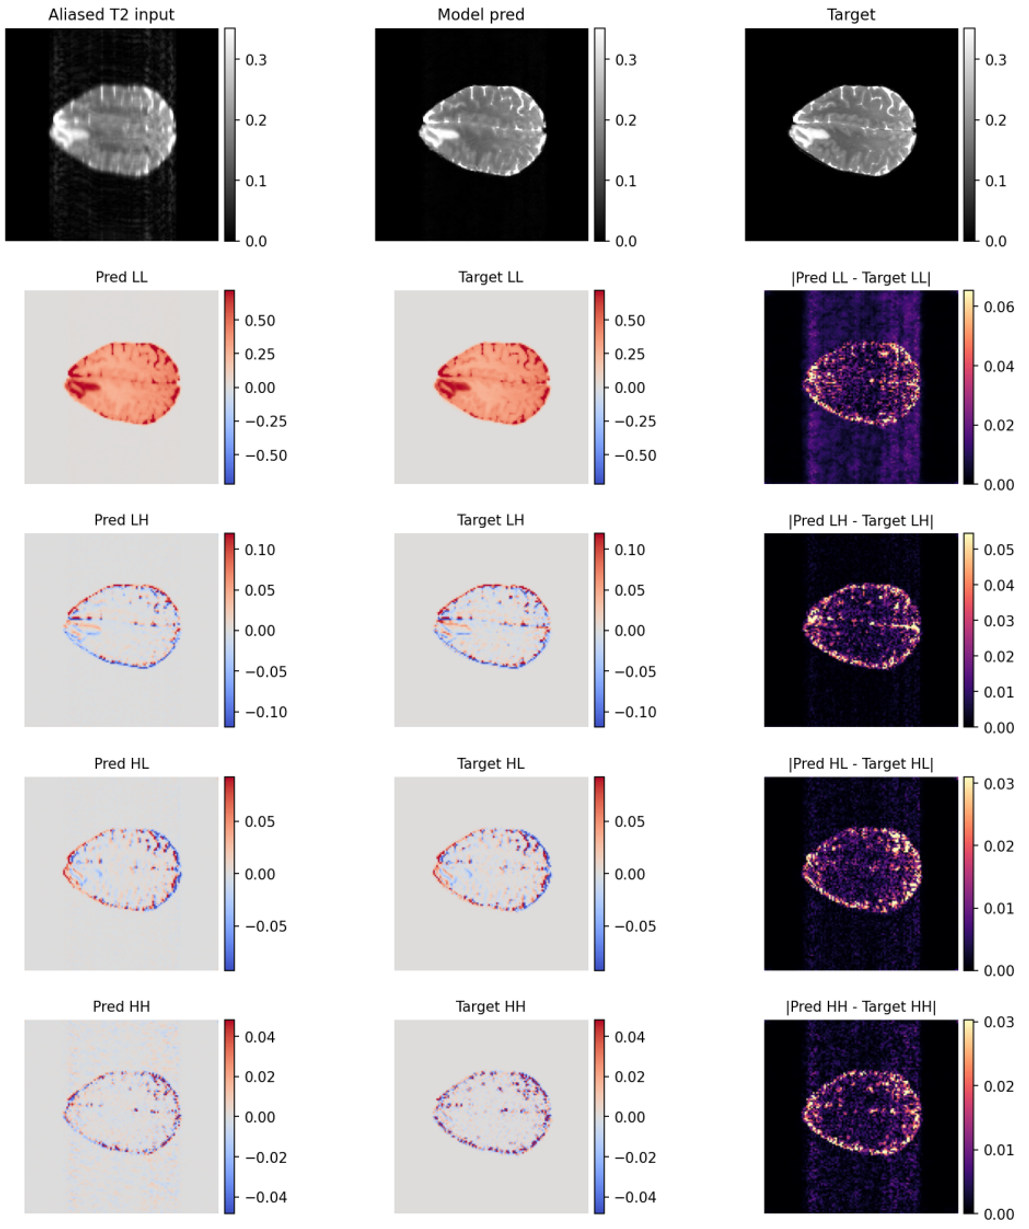
\includegraphics[width=0.8\linewidth]{figures/wavelet.png}
    \caption{Visualization of the Wavelet Loss components. The figure compares the predicted and target images across different frequency bands (LL, LH, HL, HH), highlighting the structural details captured by the high-frequency components.}
    \label{fig:wavelet_vis}
\end{figure}

\textbf{Perceptual Loss ($\mathcal{L}_{LPIPS}$):} To ensure the reconstructed image aligns with human visual perception and preserves complex texture details, we incorporated the Learned Perceptual Image Patch Similarity (LPIPS) metric as a loss function. This perceptual loss computes the distance between deep feature representations extracted by a pre-trained network, rather than simply comparing raw pixel intensities. 


\begin{figure*}[t] 
	\begin{center} 
		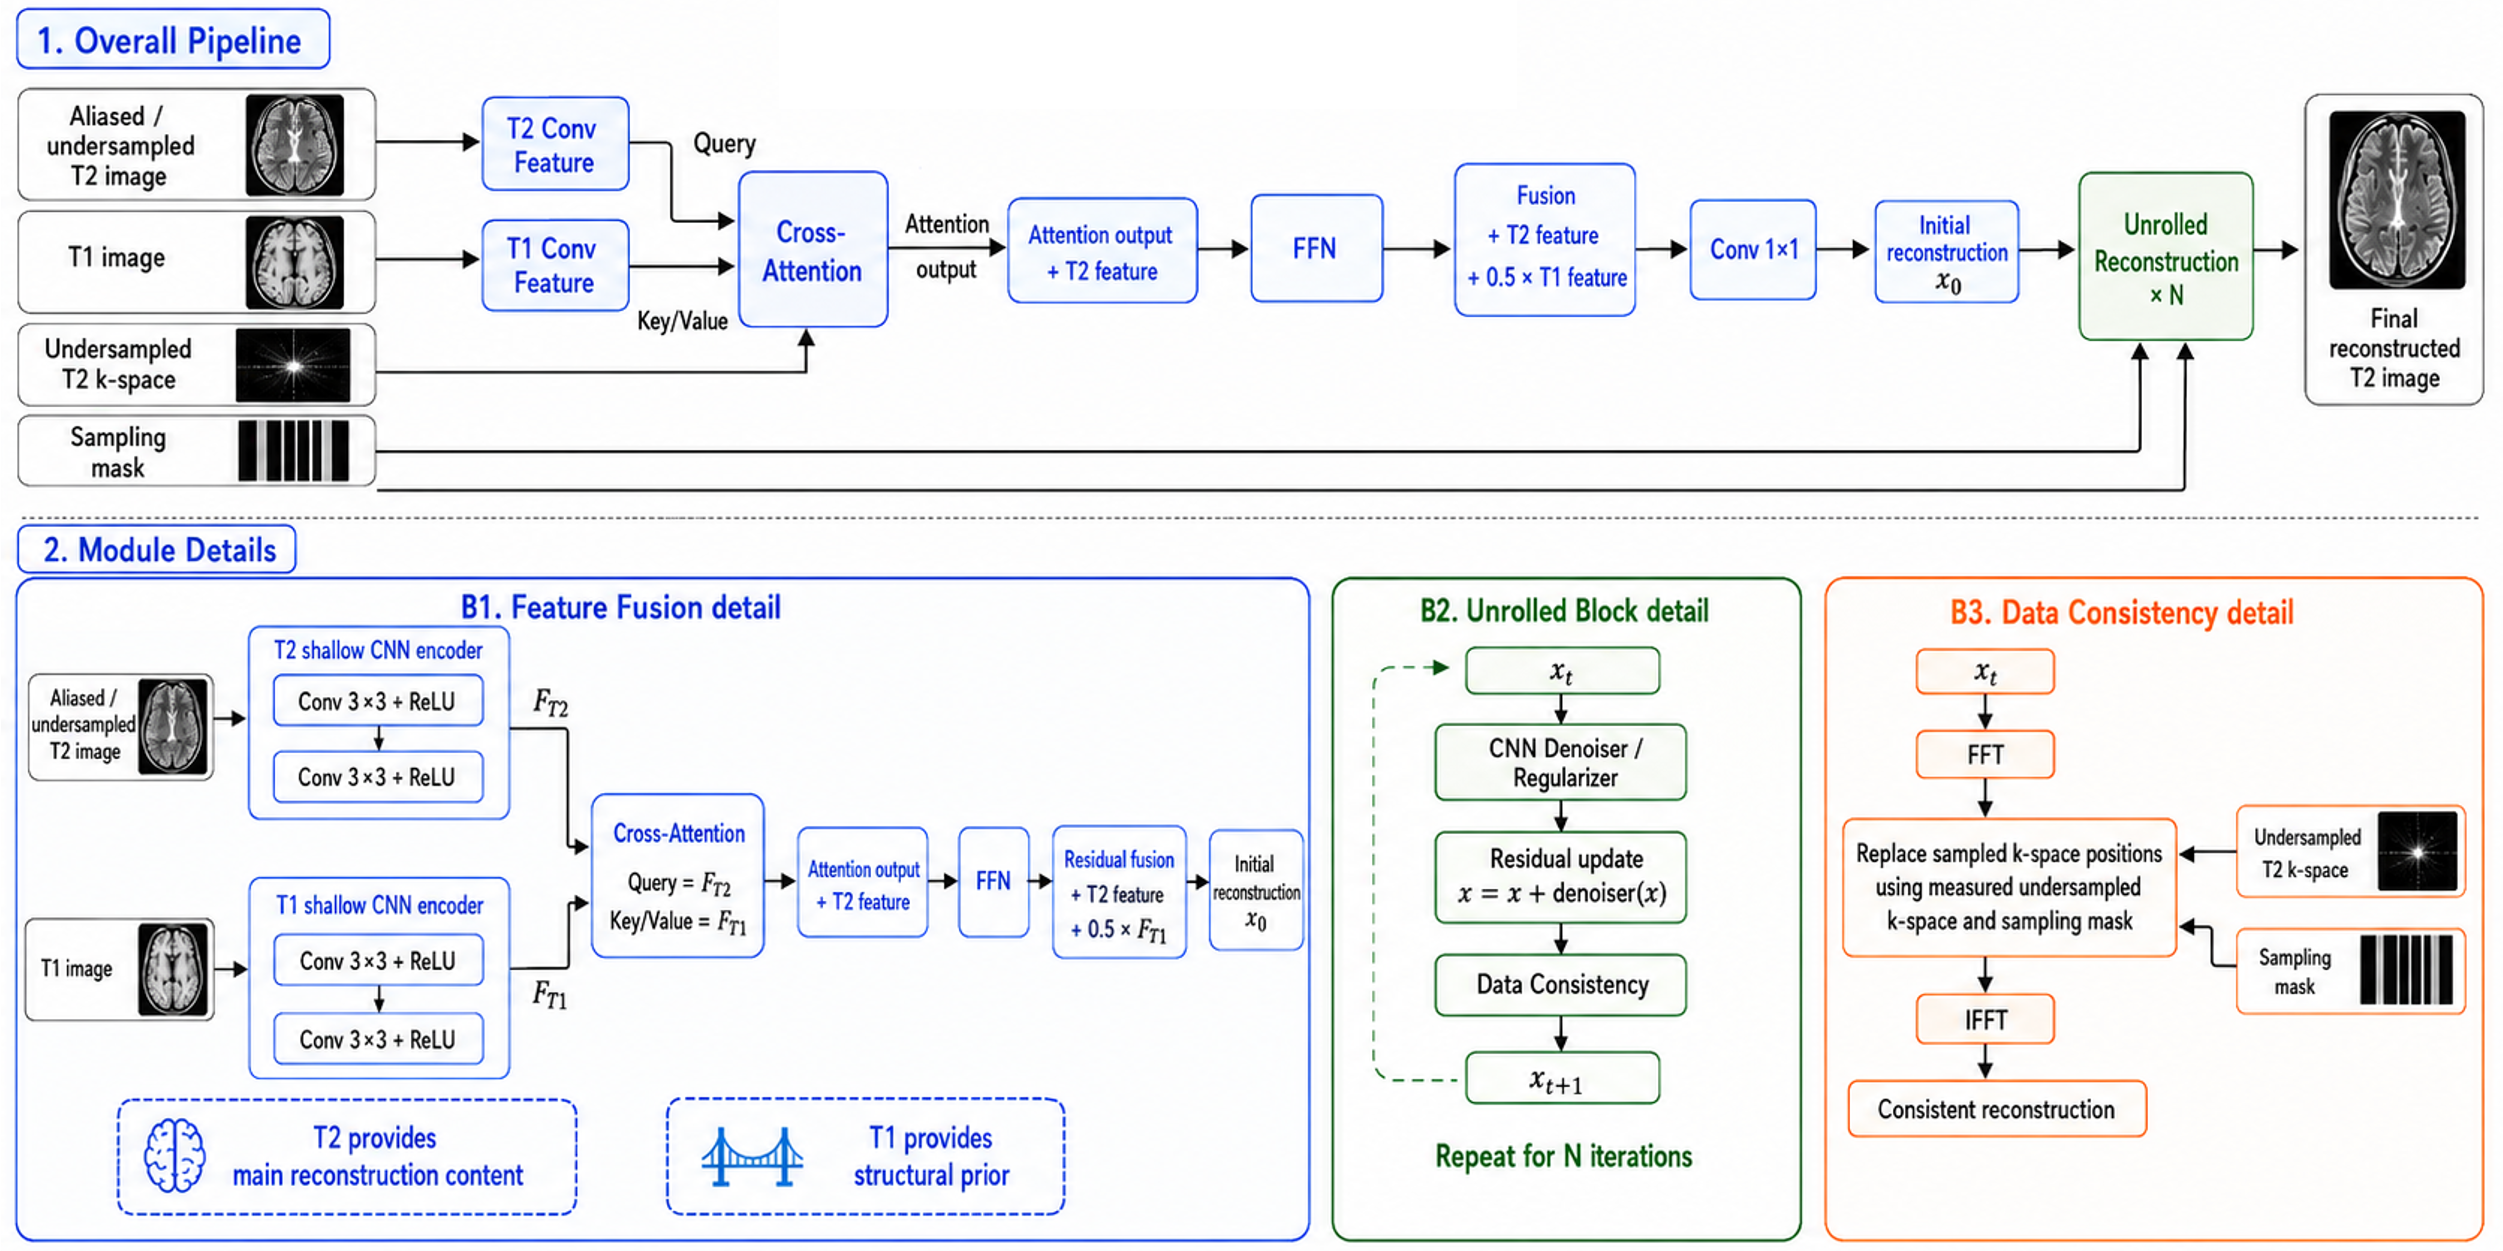
\includegraphics[width=\linewidth]{figures/pipeline_2.png} 
	\end{center} 
    \vspace{-20pt}  
	\caption{Overall pipeline of the Multi-modal Unrolled Reconstruction Network (Task 3).}
	\label{fig:task3_pipeline} 
	\vspace{-15pt}
\end{figure*}